\title{Composing Random Variables}

{{navbar}}

\subsubsection{Composing Random Variables}

Core to Edward's design is compositionality. Compositionality enables
fine control of modeling, where models are represented as a collection
of random variables.

We outline how to write popular classes of models using Edward:
directed graphical models, neural networks, Bayesian nonparametrics,
and probabilistic programs. For more examples, see the
\href{/tutorials/}{model tutorials}.

\subsubsection{Directed Graphical Models}

Graphical models are a rich formalism for specifying probability
distributions \citep{koller2009probabilistic}.
In Edward, directed edges in a graphical model are implicitly defined
when random variables are composed with one another. We illustrate
with a Beta-Bernoulli model,
\begin{equation*}
p(\mathbf{x}, \theta) =
\text{Beta}(\theta\mid 1, 1)
\prod_{n=1}^{50} \text{Bernoulli}(x_n\mid \theta),
\end{equation*}
where $\theta$ is a latent probability shared across the 50 data
points $\mathbf{x}\in\{0,1\}^{50}$.

\begin{lstlisting}[language=python]
from edward.models import Bernoulli, Beta

theta = Beta(1.0, 1.0)
x = Bernoulli(probs=tf.ones(50) * theta)
\end{lstlisting}

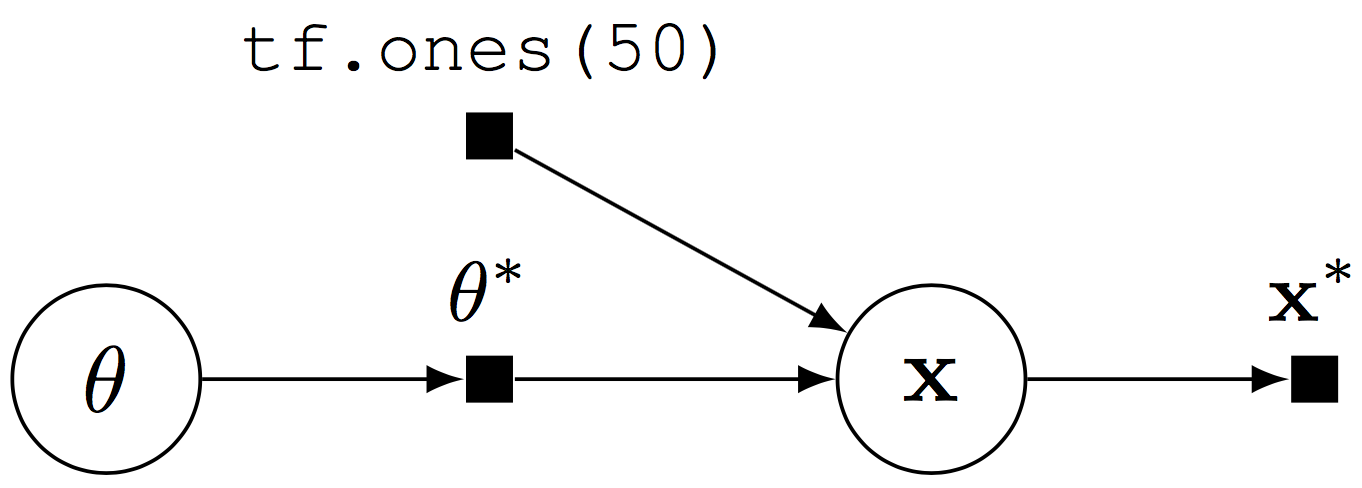
\includegraphics[width=450px]{/images/beta_bernoulli.png} \\
{\small\textit{%
Computational graph for a Beta-Bernoulli program.
}}

The random variable \texttt{x} ($\mathbf{x}$) is 50-dimensional,
parameterized by the random tensor $\theta^*$. Fetching \texttt{x}
from a session runs the graph: it simulates from the generative process
and outputs a binary vector ($\mathbf{x}^*$) of $50$ elements.

With computational graphs, it is also natural to build mutable states
within the probabilistic program. As a typical use of computational
graphs, such states can define model parameters, that is, parameters
that we will always compute point estimates for and not be uncertain
about. In TensorFlow, this is given by a \texttt{tf.Variable}.

\begin{lstlisting}[language=python]
from edward.models import Bernoulli

theta = tf.Variable(0.0)
x = Bernoulli(probs=tf.ones(50) * tf.sigmoid(theta))
\end{lstlisting}

Another use case of mutable states is for building discriminative
models $p(\mathbf{y}\mid\mathbf{x})$, where $\mathbf{x}$ are features
that are input as training or test data. The program can be written
independent of the data, using a mutable state
(\texttt{tf.placeholder}) for $\mathbf{x}$ in its graph. During
training and testing, we feed the placeholder the appropriate values.
(See the
\href{/tutorials/supervised-regression}{Bayesian linear
regression} tutorial as an example.)

\subsubsection{Neural Networks}

As Edward uses TensorFlow, it is easy to construct neural networks for
probabilistic modeling \citep{rumelhart1988parallel}.
For example, one can specify stochastic neural networks
\citep{neal1990learning}; see the
\href{/tutorials/bayesian-neural-network}{Bayesian neural network tutorial}
for details.

High-level libraries such as
\href{http://keras.io}{Keras} and
\href{https://github.com/tensorflow/tensorflow/tree/master/tensorflow/contrib/slim}{TensorFlow Slim}
can be used to easily construct deep neural networks.
We illustrate this with a deep generative model over binary data
$\{\mathbf{x}_n\}\in\{0,1\}^{N\times 28*28}$.

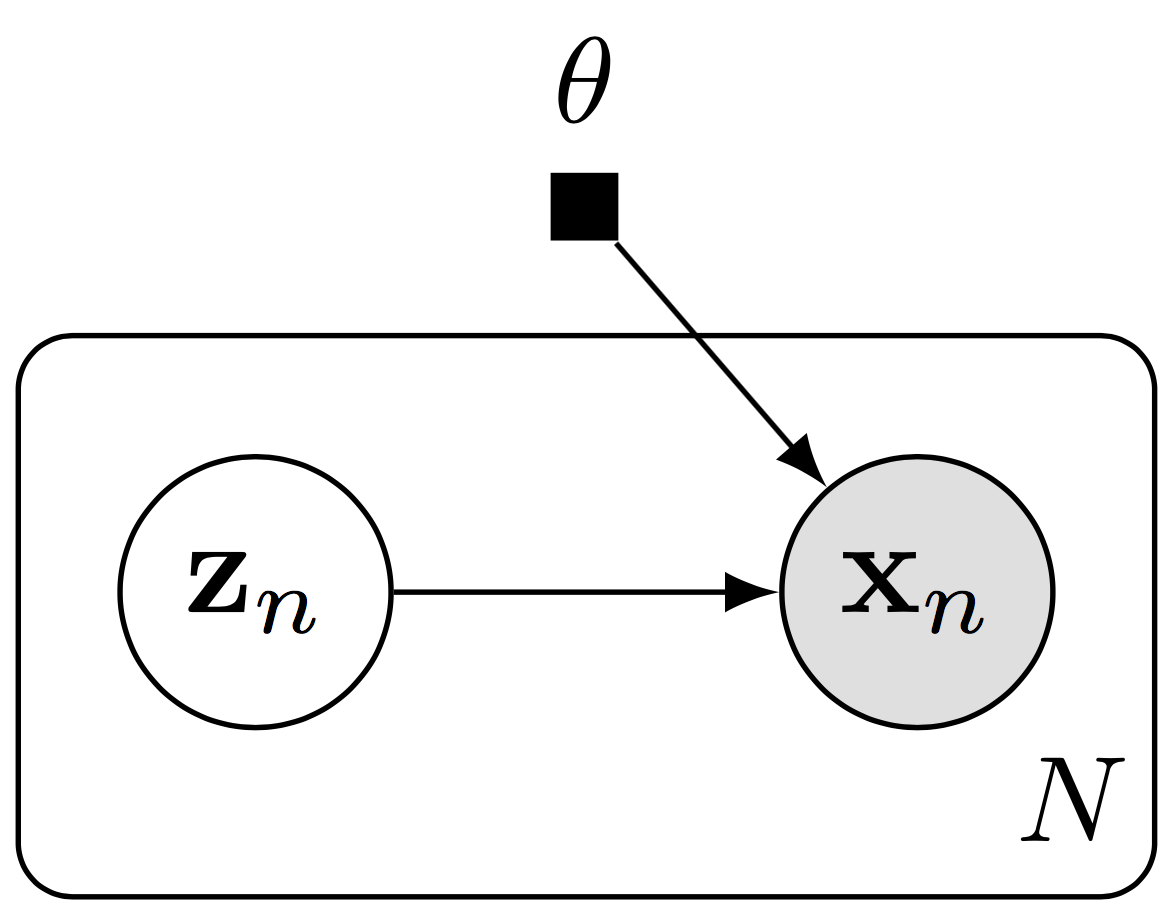
\includegraphics[width=250px]{/images/decoder.png}

{\small\textit{Graphical representation of a deep generative model.}}

The model specifies a generative process where for each
$n=1,\ldots,N$,
%
\begin{align*}
\mathbf{z}_n &\sim \text{Normal}(\mathbf{z}_n \mid \mathbf{0}, \mathbf{I}), \\[1.5ex]
\mathbf{x}_n\mid \mathbf{z}_n &\sim \text{Bernoulli}(\mathbf{x}_n\mid
p=\mathrm{NN}(\mathbf{z}_n; \mathbf{\theta})).
\end{align*}
%
The latent space is $\mathbf{z}_n\in\mathbb{R}^d$ and the
likelihood is parameterized by a neural network $\mathrm{NN}$ with
parameters $\theta$. We will use a two-layer neural network with a
fully connected hidden layer of 256 units (with ReLU activation) and
whose output is $28*28$-dimensional. The output will be unconstrained,
parameterizing the logits of the Bernoulli likelihood.

With TensorFlow Slim, we write this model as follows:

\begin{lstlisting}[language=python]
from edward.models import Bernoulli, Normal
from tensorflow.contrib import slim

z = Normal(loc=tf.zeros([N, d]), scale=tf.ones([N, d]))
h = slim.fully_connected(z, 256)
x = Bernoulli(logits=slim.fully_connected(h, 28 * 28, activation_fn=None))
\end{lstlisting}

With Keras, we write this model as follows:

\begin{lstlisting}[language=python]
from edward.models import Bernoulli, Normal
from keras.layers import Dense

z = Normal(loc=tf.zeros([N, d]), scale=tf.ones([N, d]))
h = Dense(256, activation='relu')(z)
x = Bernoulli(logits=Dense(28 * 28)(h))
\end{lstlisting}

Keras and TensorFlow Slim automatically manage TensorFlow variables, which
serve as parameters of the high-level neural network layers. This
saves the trouble of having to manage them manually. However, note
that neural network parameters defined this way always serve as model
parameters. That is, the parameters are not exposed to the user so we
cannot be Bayesian about them with prior distributions.

\subsubsection{Bayesian Nonparametrics}

Bayesian nonparametrics enable rich probability models by working over
an infinite-dimensional parameter space \citep{hjort2010bayesian}.
Edward supports the two typical approaches to handling these models:
collapsing the infinite-dimensional space and lazily defining the
infinite-dimensional space.

In the collapsed approach, we specify a distribution over its
instantiation, and the stochastic process is implicitly marginalized
out. For example, we can represent a distribution over the function
evaluations of a Gaussian process, and not explicitly represent the
function draw.

\begin{lstlisting}[language=Python]
from edward.models import Bernoulli, Normal

def kernel(X):
  """Evaluate kernel over each pair of rows (data points) in the matrix."""
  return

X = tf.placeholder(tf.float32, [N, D])
y = MultivariateNormalTriL(loc=tf.zeros(N), scale_tril=kernel(X))
\end{lstlisting}

For more details, see the
\href{/tutorials/supervised-classification}{Gaussian process classification}
tutorial. This approach is also useful for Poisson process models.

In the lazy approach, we work directly on the infinite-dimensional space via
\href{https://www.tensorflow.org/api_guides/python/control_flow_ops}{control flow operations}
in TensorFlow. At runtime, the control flow will execute only the
necessary computation in order to terminate. As an example, Edward
provides a \texttt{DirichletProcess} random variable.

\begin{lstlisting}[language=Python]
import matplotlib.pyplot as plt
from edward.models import DirichletProcess, Normal

def plot_dirichlet_process(alpha):
  with tf.Session() as sess:
    dp = DirichletProcess(alpha, Normal(0.0, 1.0))
    samples = sess.run(dp.sample(1000))
    plt.hist(samples, bins=100, range=(-3.0, 3.0))
    plt.title("DP({0}, N(0, 1))".format(alpha))
    plt.show()

# Dirichlet process with high concentration
plot_dirichlet_process(1.0)
# Dirichlet process with low concentration (more spread out)
plot_dirichlet_process(50.0)
\end{lstlisting}

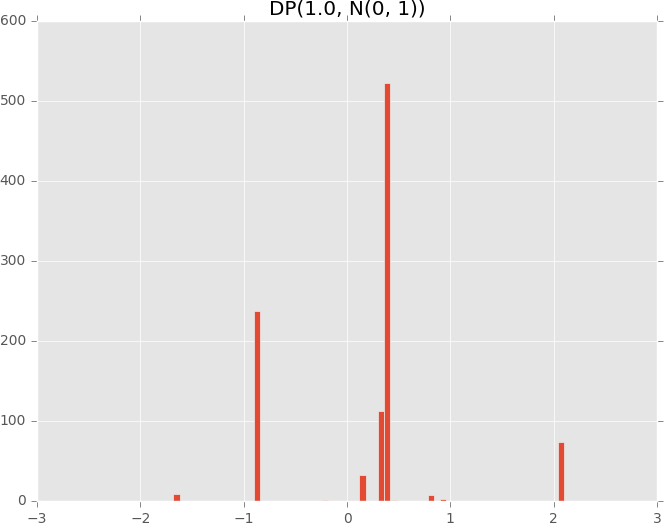
\includegraphics[width=350px]{/images/dirichlet-process-fig0.png}
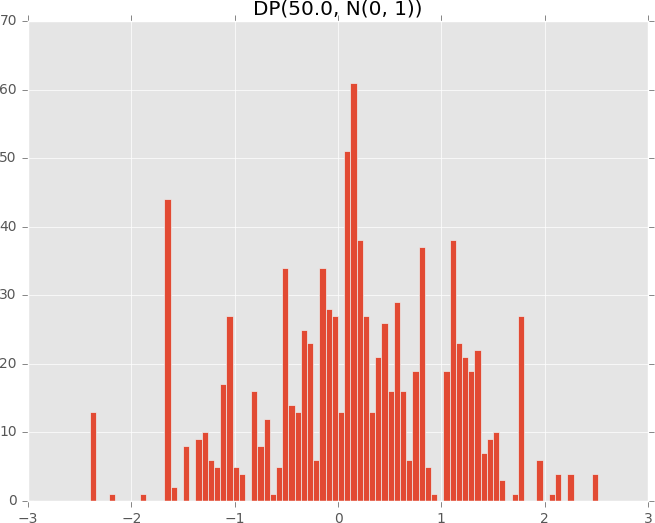
\includegraphics[width=350px]{/images/dirichlet-process-fig1.png}

To see the essential component defining the \texttt{DirichletProcess}, see
\href{https://github.com/blei-lab/edward/blob/master/examples/pp_dirichlet_process.py}{\texttt{examples/pp_dirichlet_process.py}}
in the Github repository. Its source implementation can be found at
\href{https://github.com/blei-lab/edward/blob/master/edward/models/dirichlet_process.py}{\texttt{edward/models/dirichlet_process.py}}.

\subsubsection{Probabilistic Programs}

Probabilistic programs greatly expand the scope of probabilistic
models \citep{goodman2012church}.
Formally, Edward is a Turing-complete probabilistic programming
language. This means that Edward can represent any computable
probability distribution.

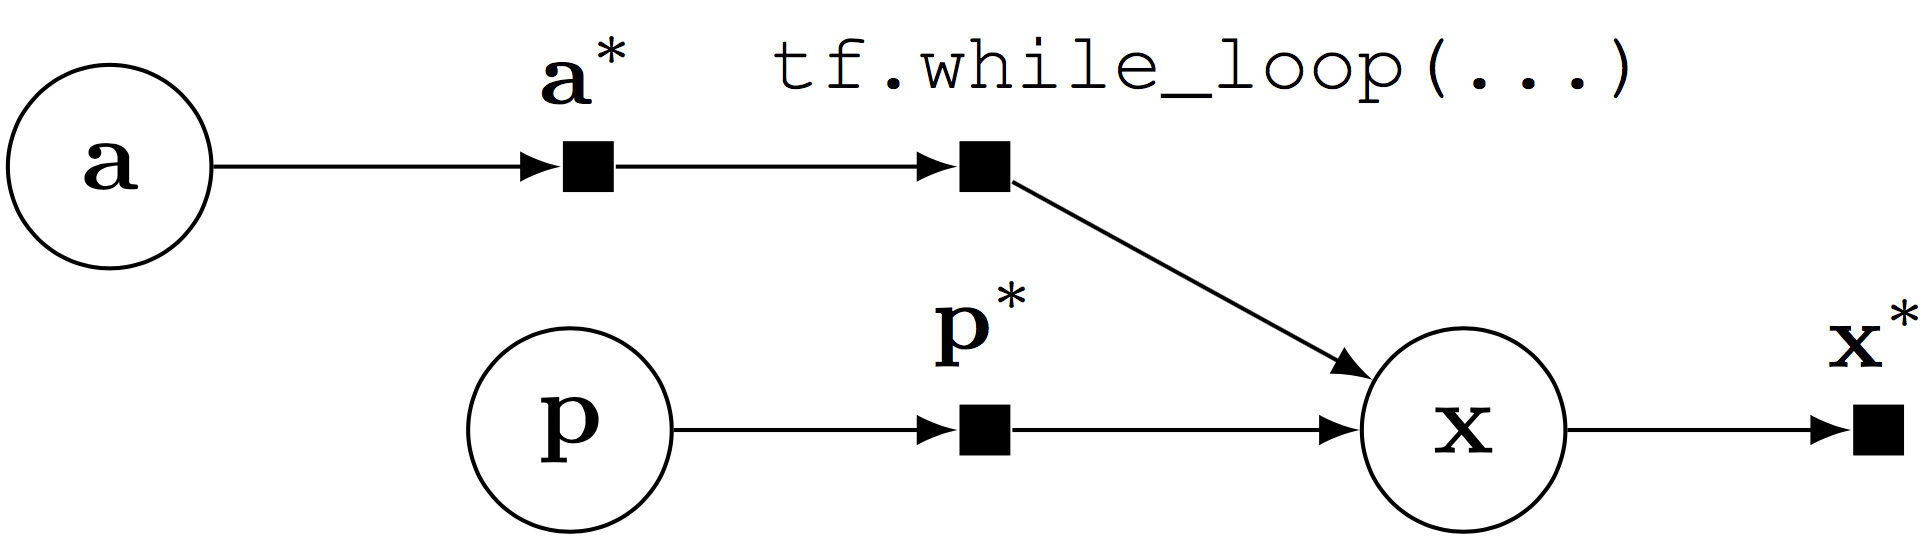
\includegraphics[width=450px]{/images/dynamic_graph.png}

{\small\textit{Computational graph for a probabilistic program with stochastic control flow.}}

Random variables can be composed with control flow operations,
enabling probabilistic programs with stochastic control flow.
%
Stochastic control flow defines dynamic conditional dependencies,
known in the literature as contingent or existential dependencies
\citep{mansinghka2014venture,wu2016swift}.
See above, where $\mathbf{x}$ may or may not depend on $\mathbf{a}$
for a given execution.

Stochastic control flow produces difficulties for algorithms that
leverage the graph structure; the relationship of conditional
dependencies changes across execution traces.
Importantly, the computational graph provides an elegant way of
teasing out static conditional dependence structure ($\mathbf{p}$)
from dynamic dependence structure ($\mathbf{a})$. We can perform
model parallelism over the static structure with GPUs and batch
training, and use generic computations to handle the dynamic
structure.

\subsubsection{References}\label{references}
